\chapter{A Recursive Technique}

In the previous chapter, we examined some structures in grids that, if present, immediately guarantee lethality. Most significantly, we proved that lethal sets on mutually orthogonal walls of a grid are lethal on the entire grid. In the following sections, we leverage this result to show that certain configurations of fully infected sub-grids (which we shall call blocks) will cause the larger grid to become infected. Furthermore, we show that if each of these smaller blocks is infected with a minimum lethal set, the composite larger brick will also be infected with a minimum lethal set (barring some considerations for divisibility).

The proof of this claim makes use of the so-called \emph{modified bootstrap process} in $[n]^d$, discussed in \cite{some paper} and \cite{some other paper}. This is a strengthened variation of the problem introduced in Chapter 1, whereby vertices in the $[n]^d$ grid become infected if and only if they are adjacent to infected vertices along edges in each of the $d$ directions. For example, in the $[n]^2$ grid, a vertex that sees infection in one of both the North/South and East/West directions will itself become infected, whereas a vertex with infected neighbors to the East and West (but not North and South) will not. 

In particular, the following lemma considers composite grids $[n]^d$ where each vertex $x = (x_1, \dots, x_d) \in [n]^d$ is itself a smaller block $G_x$. We prove that lethal sets on these grids can be built from the smaller lethal sets on each $G_x$. 
% $[b_1] \times [b_2] \times \cdots \times [b_d]$ grid

\begin{figure}[]
\centering
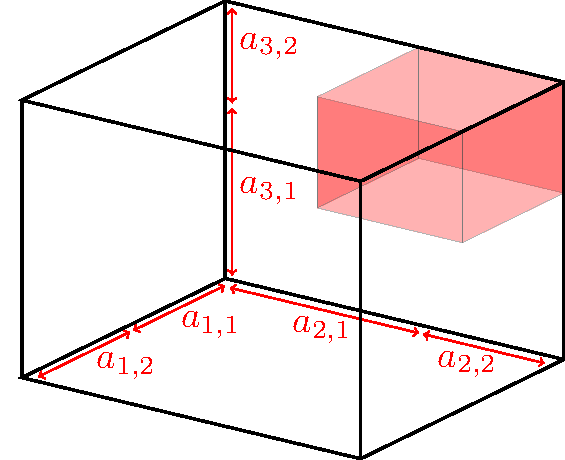
\includegraphics[width=0.4\textwidth]{figures/3/recursion.pdf}
\caption{A recursively constructed $[b_1] \times [b_2] \times [b_3]$ grid, for $n = 2$, $d = 3$.}
\label{fig:recursion}
\end{figure} 

\begin{lem}
\label{lem:recursion}
For $n,d \geq 1$, let $A = (a_{i,j})$ be a $d \times n$ matrix of positive integers, and let $b_i = \sum_{j=1}^n a_{i,j}$, for $1 \geq j \geq d$. Let $S$ be a lethal set under the modified process on $[n]^d$, and for each vertex $\vec{x} = (x_1, \dots, x_v) \in S$, let $T_{\vec{x}}$ be a lethal set on $\prod_{i=1}^d [a_{i,x_i}]$ under $d$-neighbor percolation. Then
$$m(b_1, \dots, b_d, d) \leq \sum_{\vec{x} \in S} |T_{\vec{x}}|.$$
\end{lem}

\begin{proof}
We imagine sub-dividing the $\prod_{i=1}^d [b_{i}]$ brick into smaller blocks by partitioning each of the $d$ axes into segments $a_{i,1}, a_{i,2}, \dots, a_{i,n}$, $1 \leq i \leq d$. Each block is given by a unique product of these segments, and represented by a vector $\vec{x} = (x_1, \dots, x_d) \in [n]^d$. Formally, for each such $\vec{x}$, let $G_{\vec{x}}$ be the block with vertex set
$$\prod_{i=1}^d \{1+ \sum_{j=1}^{x_i -1}a_{i,j}, \dots, \sum_{j=1}^{x_i}a_{i,j} \},$$
and edges between vertices that differ by one in exactly one coordinate. Figure \ref{fig:recursion} illustrates the block $G_{\vec{x}}$ for $\vec{x} = (1,2,2) \in [2]^3$. Observe that $G_{\vec{x}}$ is isomorphic to $\prod_{i=1}^d [a_{i,x_i}]$.

For each $\vec{x} \in S$, let $A_{\vec{x}}$ be the vertices of $G_{\vec{x}}$ corresponding to the vertices of $T_{\vec{x}}$ under isomorphism from $\prod_{i=1}^d [a_{i,x_i}]$ to $G_{\vec{x}}$, and let $A_0 = \cup A_{\vec{x}}$. Observe that $|A_0| = \sum_{\vec{x} \in S} |T_{\vec{x}}|$. We show that $A_0$ is lethal on $\prod_{i=1}^d [b_{i}]$.

By the definition of $T_{\vec{x}}$, for each $\vec{x} \in S$, $A_{\vec{x}}$ is lethal on $G_{\vec{x}}$. Imagine running the $d$-neighbor process until all blocks $G_{\vec{x}}$ are fully infected. We claim that this is sufficient to infect all remaining vertices of $\prod_{i=1}^d [b_{i}]$. Consider the remaining blocks $G_{\vec{x}}$, for $\vec{x} \in [n]^d \setminus S$. Since $S$ is lethal under the modified process, each $G_{\vec{x}}$ is adjacent to fully infected blocks in all $d$ directions. In particular, if we consider expanding out the faces of $G_{\vec{x}}$ towards these infected blocks, the resulting cube has $d$ fully infected faces that share a common corner. By Corollary \ref{cor:three_walls}, this structure will infect all the vertices of $G_{\vec{x}}$. Repeating this process on each uninfected region of $\prod_{i=1}^d [b_{i}]$ (as they are exposed under the modified process) ultimately results in all vertices becoming infected. This completes the proof. 
\end{proof}

% Corollary that shows the recursion produces tight bounds on the size of lethal sets, IF all of the constituent blocks are divisibility cases
We note that although the lemma above is true in full generality, we are only concerned with the particular case where $n=2$ and $d=3$. The following corollary proves that the bound in Lemma \ref{lem:recursion} is tight for $n=2$ and $d=3$, if lethal sets on at least three of the constituent blocks are perfect. 

\begin{cor}
\label{cor:recursion}
Let $A=(a_{i,j})$ be a $3 \times 2$ matrix of positive integers, and let $b_i = a_{i,1} + a_{i,2}$ for all $1 \leq i \leq 3$. Then $m(b_1, b_2, b_3, 3)$ is at most
$$m(a_{1,1}, a_{2,1}, a_{3,1}, 3) +  m(a_{1,2}, a_{2,2}, a_{3,1}, 3) + m(a_{1,2}, a_{2,1}, a_{3,2}, 3) + m(a_{1,1}, a_{2,2}, a_{3,2}, 3).$$
Furthermore, this bound is tight if at least 3 of the constituent grids are perfect. 
\end{cor}

\begin{proof}
The upper bound on $m(b_1, b_2, b_3, 3)$ is a direct consequence of Lemma \ref{lem:recursion}, since $(1,1,1), (2,2,1), (2,1,2), (1,2,2)$ is lethal under the modified process on $[2]^3$. 

If all grids are perfect, then:  
\begin{align*}
&m(a_{1,1}, a_{2,1}, a_{3,1}, 3) +  m(a_{1,2}, a_{2,2}, a_{3,1}, 3) + m(a_{1,2}, a_{2,1}, a_{3,2}, 3) + m(a_{1,1}, a_{2,2}, a_{3,2}, 3) \\[10pt]
&= \frac{a_{1,1}a_{2,1} + a_{2,1}a_{3,1} + a_{3,1}a_{1,1}}{3} + \frac{a_{1,2}a_{2,2} + a_{2,2}a_{3,1} + a_{3,1}a_{1,2}}{3} \\
&\qquad\qquad\qquad\qquad\qquad\qquad\quad + \frac{a_{1,2}a_{2,1} + a_{2,1}a_{3,2} + a_{3,2}a_{2,1}}{3} + \frac{a_{1,1}a_{2,2} + a_{2,2}a_{3,2} + a_{3,2}a_{1,1}}{3} \\[10pt]
&= \frac{(a_{1,1} + a_{1,2})(a_{2,1} + a_{2,2}) + (a_{2,1} + a_{2,2})(a_{3,1} + a_{3,2}) + (a_{3,1} + a_{3,2})(a_{1,1} + a_{1,2})}{3} \\[10pt]
&= \frac{b_1b_2+b_2b_3+b_3b_1}{3}.
\end{align*}
Similarly, suppose, without loss of generality, that $(a_{1,1}, a_{2,1}, a_{3,1})$ is optimal and the remaining grids are perfect. Then:
\begin{align*}
&m(a_{1,1}, a_{2,1}, a_{3,1}, 3) +  m(a_{1,2}, a_{2,2}, a_{3,1}, 3) + m(a_{1,2}, a_{2,1}, a_{3,2}, 3) + m(a_{1,1}, a_{2,2}, a_{3,2}, 3) \\[10pt]
&= \ceil*{\frac{a_{1,1}a_{2,1} + a_{2,1}a_{3,1} + a_{3,1}a_{1,1}}{3}} + \frac{a_{1,2}a_{2,2} + a_{2,2}a_{3,1} + a_{3,1}a_{1,2}}{3} \\
&\qquad\qquad\qquad\qquad\qquad\qquad\quad + \frac{a_{1,2}a_{2,1} + a_{2,1}a_{3,2} + a_{3,2}a_{2,1}}{3} + \frac{a_{1,1}a_{2,2} + a_{2,2}a_{3,2} + a_{3,2}a_{1,1}}{3} \\[10pt]
&= \ceil*{\frac{(a_{1,1} + a_{1,2})(a_{2,1} + a_{2,2}) + (a_{2,1} + a_{2,2})(a_{3,1} + a_{3,2}) + (a_{3,1} + a_{3,2})(a_{1,1} + a_{1,2})}{3}} \\[10pt]
&= \ceil*{\frac{b_1b_2+b_2b_3+b_3b_1}{3}}.
\end{align*}
In both cases, we obtain the lower bound $m(b_1, b_2, b_3, 3)$. This completes the proof. 
\end{proof}

\section{Applying the recursion}

\begin{table}[]
\centering
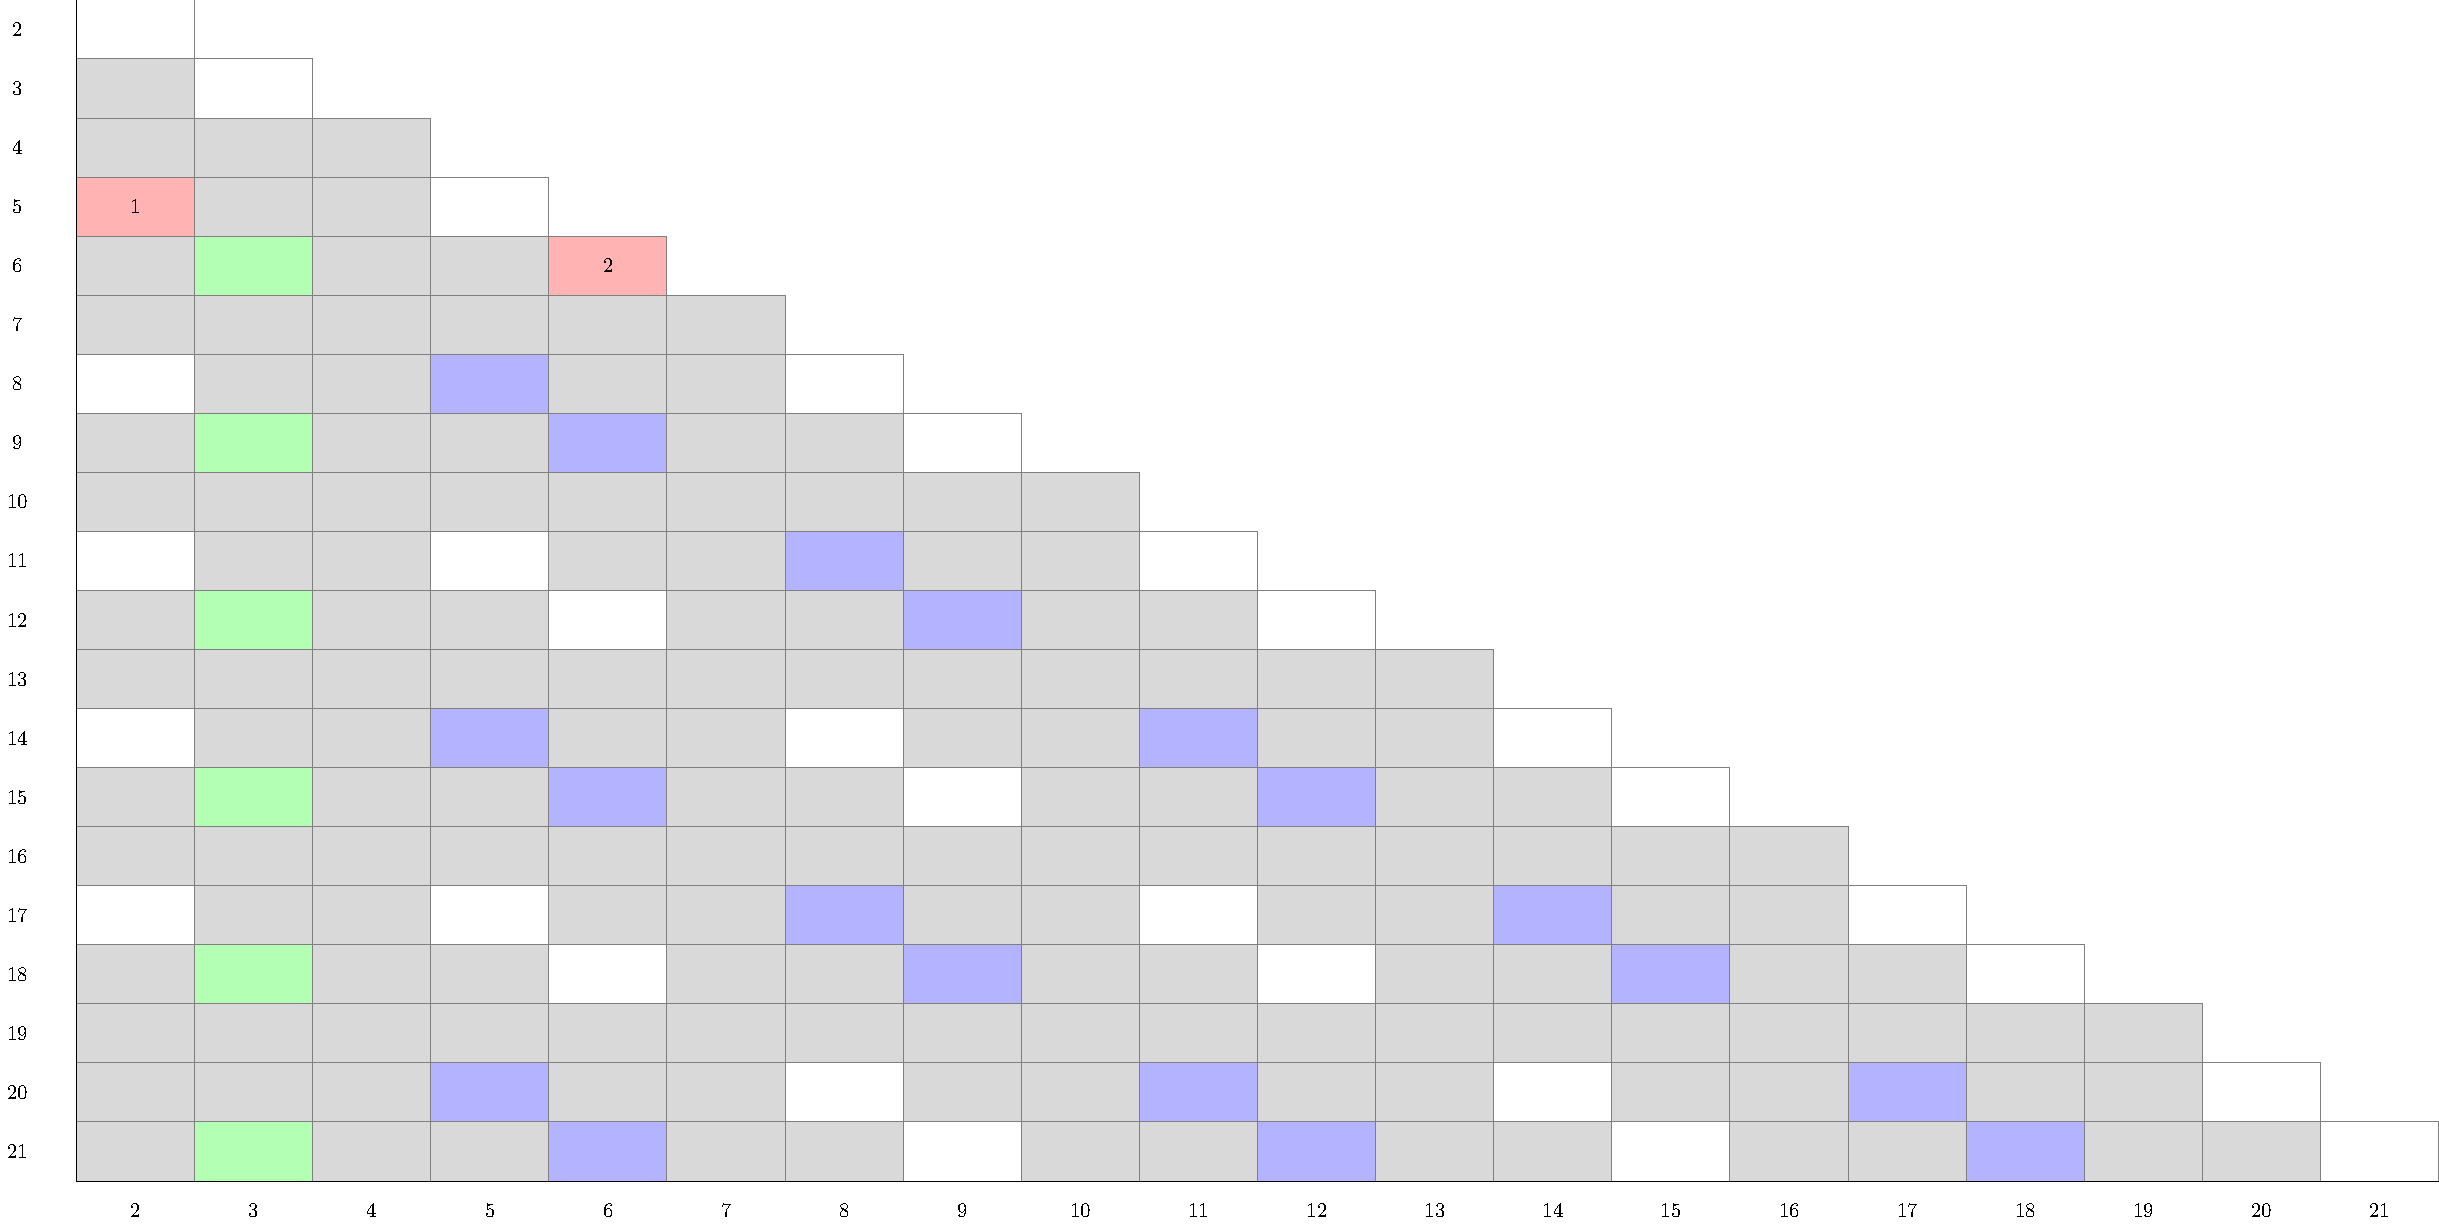
\includegraphics[width=\textwidth]{tables/2/thickness_2.pdf}
\caption{Thickness 2 constructions used in the proof of Theorem \ref{thm:main_result}. Blue and green cells represent infinite families of constructions. Red cells are individual constructions. Divisibility cases are white and non-divisibility cases are gray.}
\label{tab:integral_bounds_2}
\end{table} 

\begin{table}[]
\centering
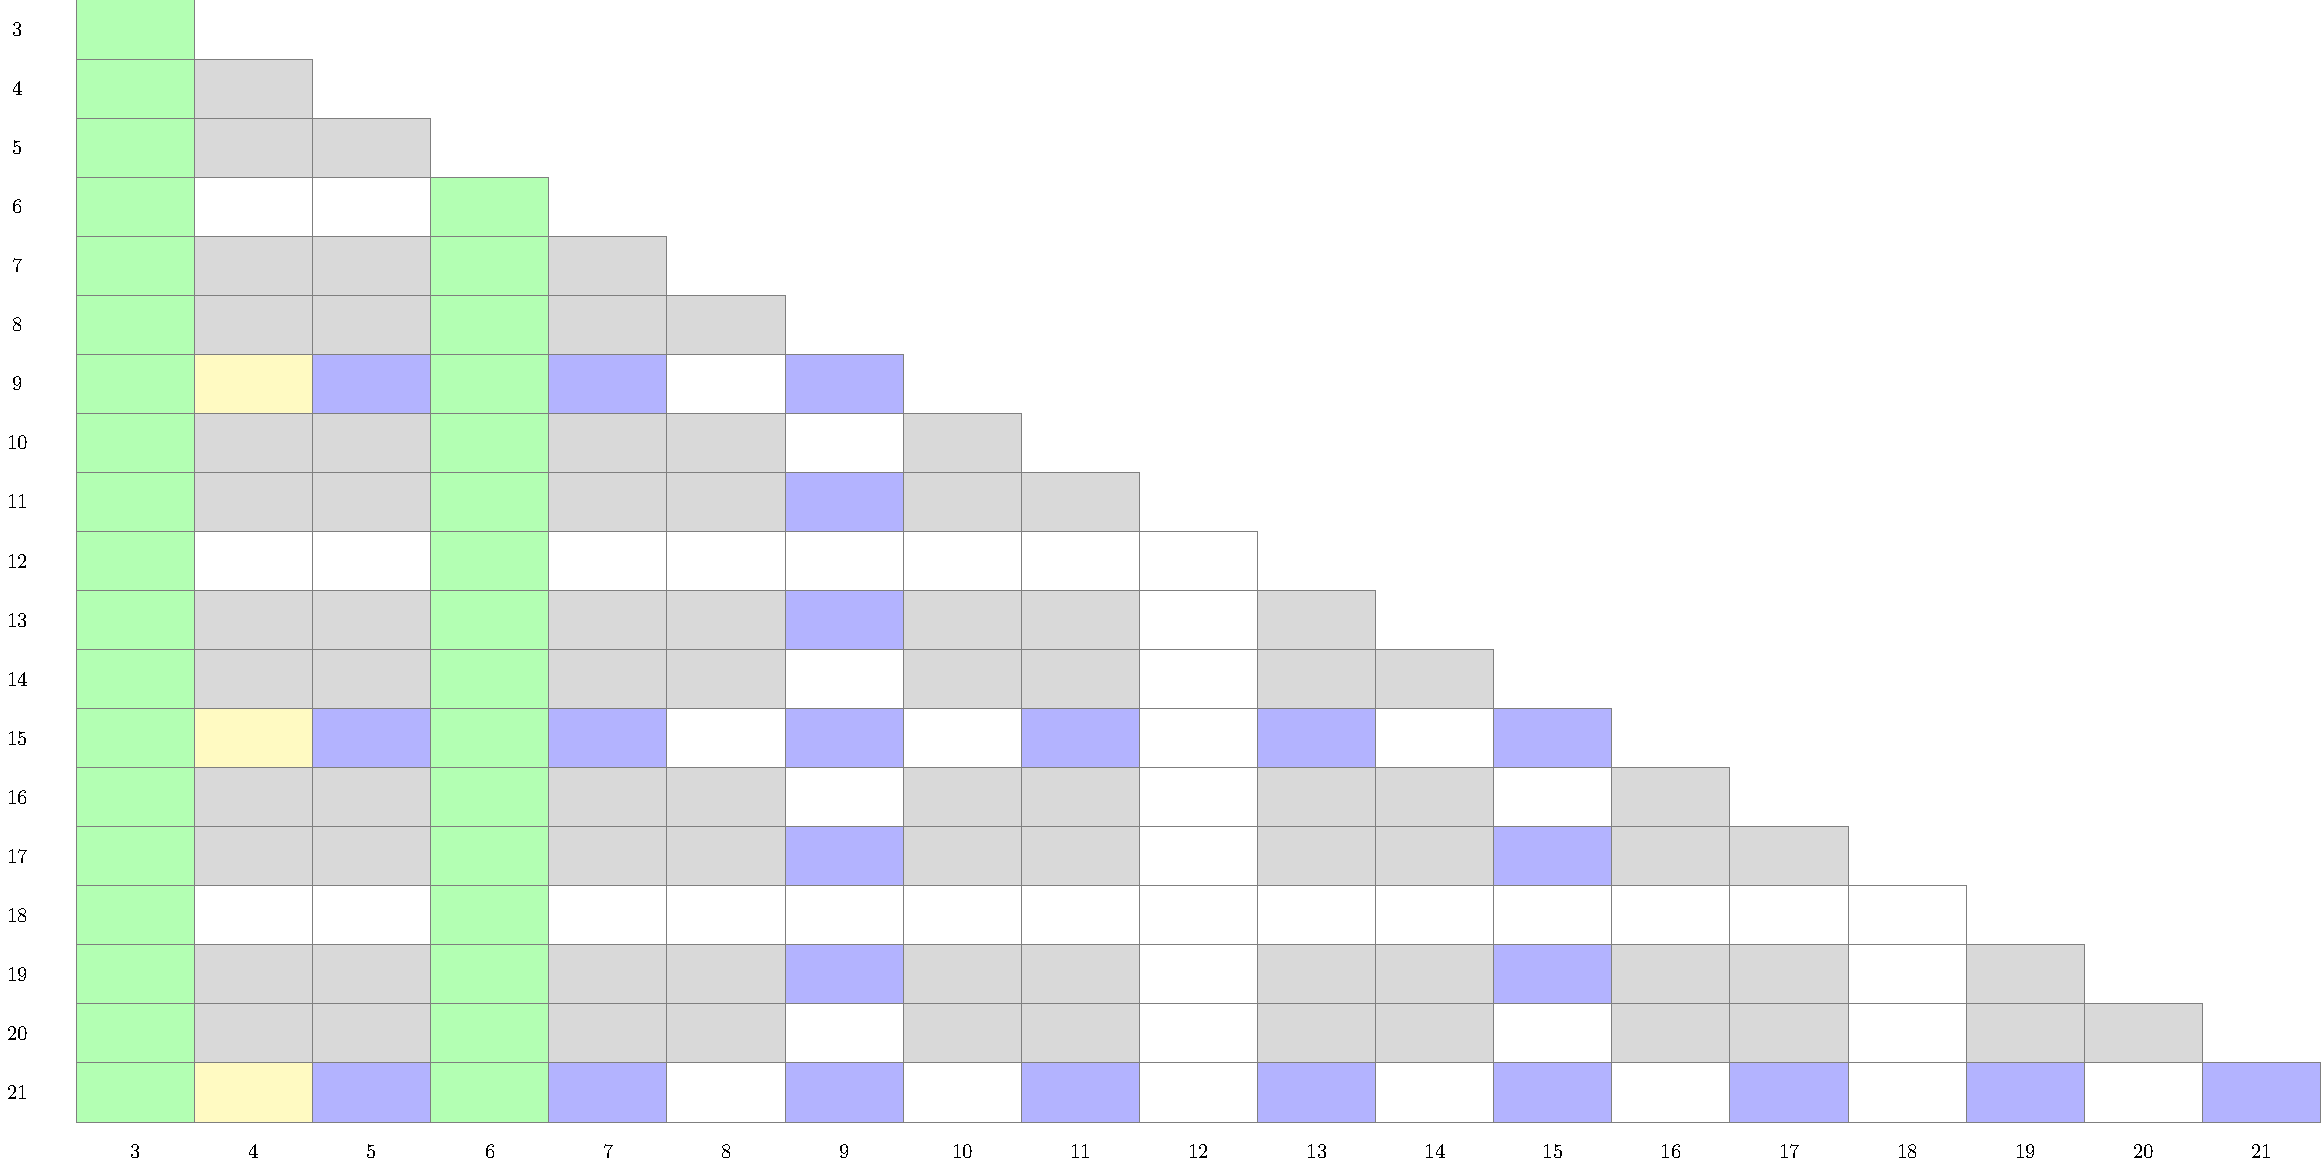
\includegraphics[width=\textwidth]{tables/2/thickness_3.pdf}
\caption{Thickness 3 constructions used in the proof of Theorem \ref{thm:main_result}. Blue, green and yellow cells represent infinite families of constructions. Red cells are individual constructions. Divisibility cases are white and non-divisibility cases are gray.}
\label{tab:integral_bounds_3}
\end{table} 

\begin{table}[]
\centering
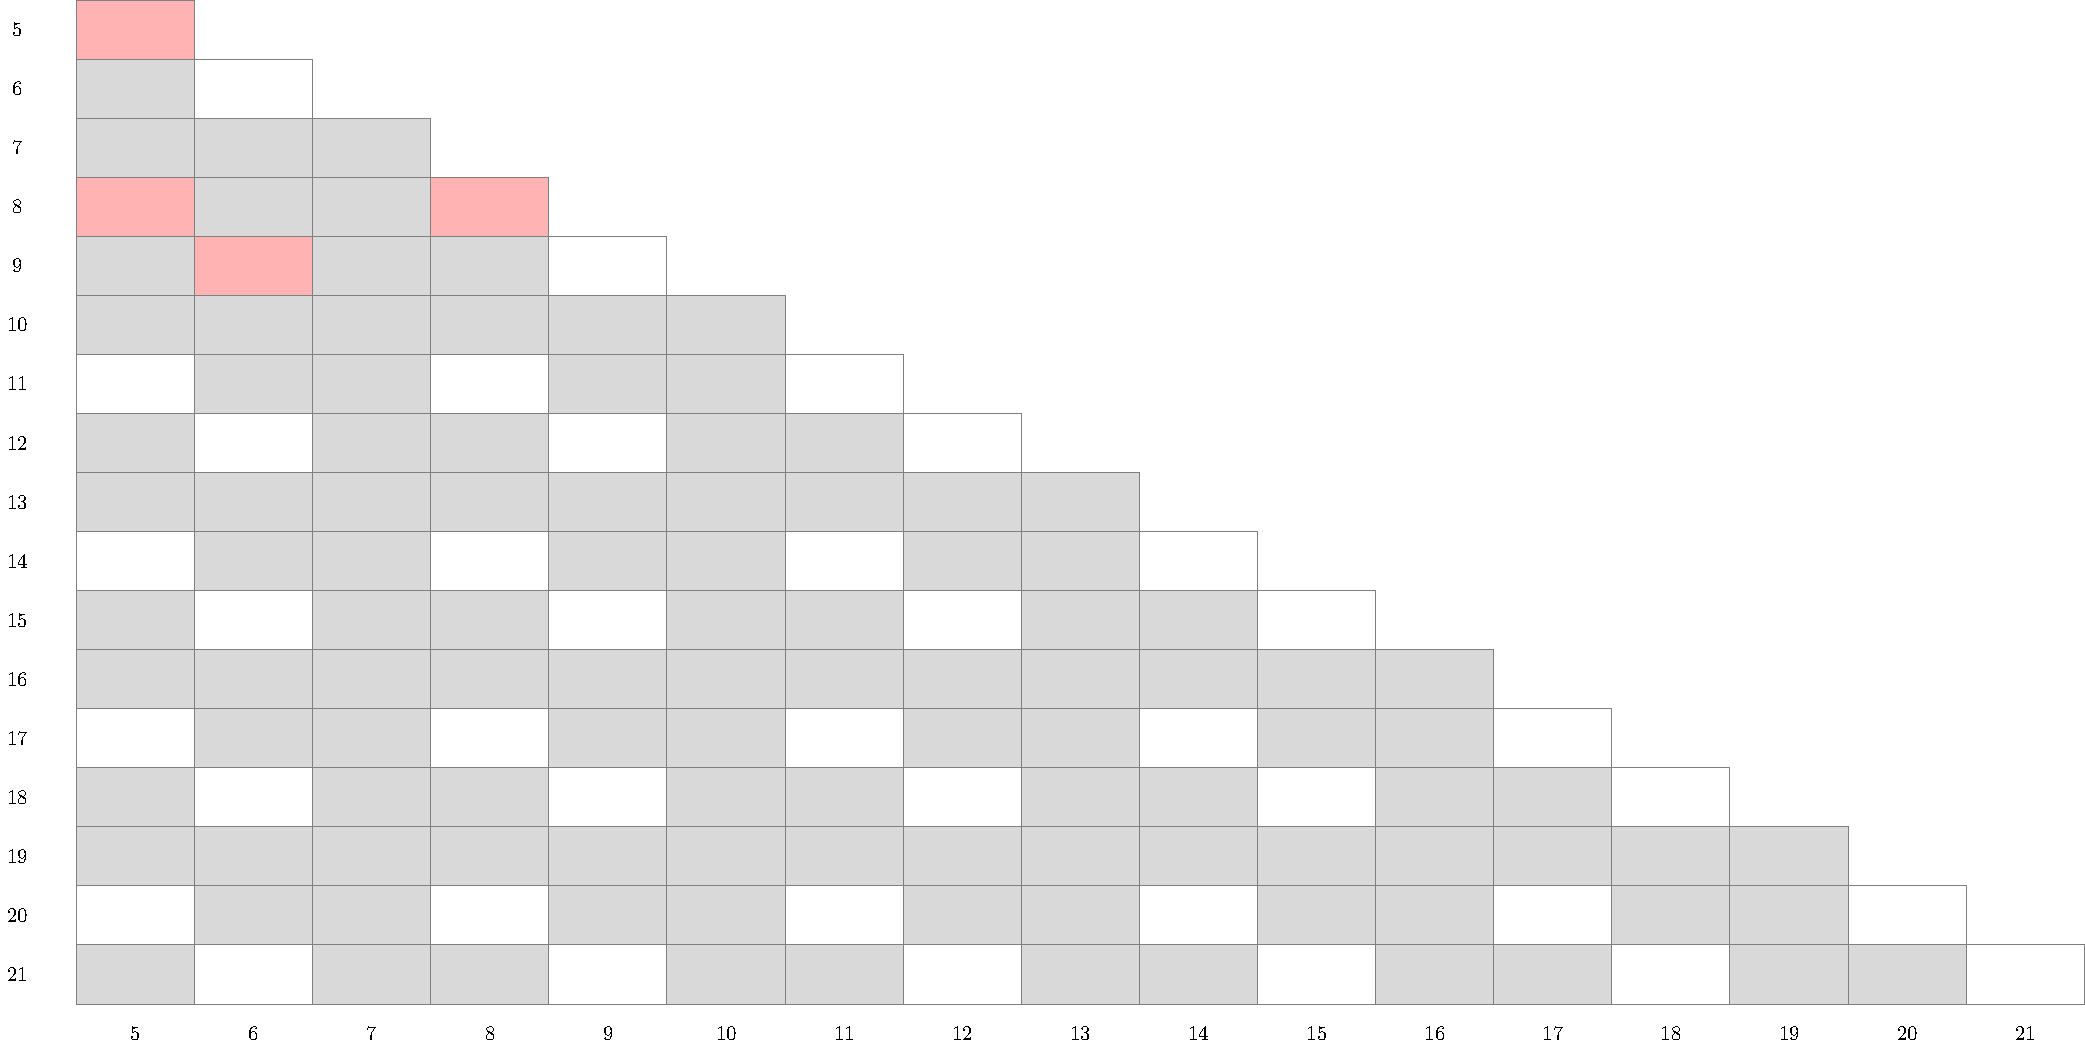
\includegraphics[width=\textwidth]{tables/2/thickness_5.pdf}
\caption{Thickness 5 constructions used in the proof of Theorem \ref{thm:main_result}. Red cells are individual constructions. Divisibility cases are white and non-divisibility cases are gray.}
\label{tab:integral_bounds_5}
\end{table}

% Handle the divisibility cases, and note that certain augmentations to the recursion allow us to obtain non-divisible optimal grids, if we are cautious with regard to the pieces we use.
Corollary \ref{cor:recursion} provides a prescriptive method for constructing optimal and perfect lethal sets recursively, provided the existence of sufficiently many small building blocks. In the following chapter, we use this technique to obtain perfect lethal sets on all $(b_1,b_2,b_3)$ grids, for $b_1,b_2,b_3 \geq 5$, and optimal lethal sets on all $(b_1,b_2,b_3)$ grids, for $b_1,b_2,b_3 \geq 11$. To facilitate this process, we first summarize some useful families of lethal sets (discussed in greater detail in Chapter [Constructions] and illustrated in Tables \ref{tab:integral_bounds_2}, \ref{tab:integral_bounds_3}, and \ref{tab:integral_bounds_5}), as well as particular applications of Corollary \ref{cor:recursion} that hold for general grids. 

\begin{prop}
\label{prop:3x3xk}
For all $k \geq 1$ such that $k \neq 2$, $(3,3,k)$ is perfect.
\end{prop}

\begin{prop}
\label{prop:3x6xk}
For all $k \geq 2$, $(3,6,k)$ is perfect.
\end{prop}

\begin{prop}
\label{prop:thickness_3_2d_family}
For all $k \equiv 3 \pmod 6$ and $l \equiv 1 \pmod 2$ such that $l >1$, $(3,k,l)$ is perfect.
\end{prop}

\begin{prop}
\label{prop:thickness_2_2d_family}
For all $k,l \in \{0,2,3,5\} \pmod 6$ such that $k \not\equiv l \pmod 6$ and $k,l > 2$, $(k,l,2)$ is perfect.
\end{prop}

\begin{prop}
\label{prop:thickness_3_width_4}
For all $k \equiv 3 \pmod 6$, $(k,4,3)$ is perfect.
\end{prop}

\begin{prop}
\label{prop:2x3xk_0}
For all $k \equiv 0 \pmod 6$ such that $k>3$, $(k,2,3)$ is perfect.
\end{prop}

\begin{prop}
\label{prop:2x3xk_3}
For all $k \equiv 3 \pmod 6$ such that $k>3$, $(k,2,3)$ is perfect.
\end{prop}

\begin{prop}
\label{prop:purina}
For all $k \geq 1$, $(2^k-1,2^k-1,1)$ is perfect.
\end{prop}

Combining the above propositions with Corollary \ref{cor:recursion}, we are able to obtain the following lemmas.

\begin{lem}
\label{lem:plus_333}
Suppose $(b_1, b_2, b_3)$ is optimal. Then $(b_1+3, b_2+3, b_3+3)$ is optimal. 
\end{lem}

\begin{proof}
By Proposition \ref{prop:3x3xk}, each of $(b_1,3,3), (3,b_2,3),(3,3,b_3)$ is perfect. Therefore, by Corollary \ref{cor:recursion}, 
$$m(b_1+3, b_2+3, b_3+3, 3) = m(b_1,b_2,b_3,3) + m(b_1,3,3,3) + m(3,b_2,3,3) + m(3,3,b_3,3),$$
and so $(b_1+3, b_2+3, b_3+3)$ is optimal.
\end{proof}

% Example of the recursion on a small grid and discussion re: the strategies for analyzing percolating sets

\section{Examples and Notation}

% Discuss that the recursion works by assembling any set of compatible n^2 blocks, although it is very rare that it is necessary to use more than 4. 
% Talk about the component pieces necessary to assemble a brick of size (a,b,c).

% Should we talk about the broad behavior of percolating sets?
\section{Regional vs. Temporal Infections}

% COMMENT
% COMMENT
% COMMENT

\begin{comment}

\section{The Three Walls Lemma}

\begin{lem}
\label{lem:walls}
Let $S$ be an infected set on $G = \prod_{i=1}^d [a_i]$. Let $\overline{S} = V(G) \setminus S$, and let $H = G[\overline{S}]$ be the subgraph of $G$ induced by $\overline{S}$. For $1 \leq k \leq a_j$, let $F_{j,k} = \prod_{i=1}^{j-1} [a_i] \times \{k\} \times \prod_{i=j+1}^{d} [a_i]$ be the $k$th face of $G$ in the $j$th dimension. If $H$ does not contain a path between $F_{j,1}$ and $F_{j,a_j}$, for all $1 \leq j \leq d$, then $S$ is lethal on $G$ under $d$-neighbor percolation.
\end{lem}

\begin{proof}
We proceed by induction on $|V(H)| = \prod_{i=1}^d a_i - |S|$. If $|V(H)| = 0$, then all vertices of $G$ are infected and we are done. Suppose $|V(H)| > 0$, and consider a connected component $Y$ of $H$. By hypothesis, for all $j \in [d]$, either $V(Y) \cap F_{j,1} = \emptyset$ or $V(Y) \cap F_{j,a_j} = \emptyset$ (or both). Suppose, without loss of generality, that $V(Y) \cap F_{j,a_j} = \emptyset$.
%Since $V(H) > 0$, there exists a $k_j < a_j$ such that $V(Y) \cap F_{j,k_j}$ is non-empty. 
For each $j \in [d]$, let $x_j$ be the maximum value such that $V(Y) \cap F_{j,x_j}$ is non-empty. Note that such an $x_j$ must exist since $|V(H)| > 0$. 

Consider the vertex $\vec{x} = (x_1, \dots, x_d) \in V(Y)$, and observe that 
$$\{\bigcup_{j \in [d]} F_{j,x_j+1}\} \cap  V(Y) = \emptyset.$$
In particular, note that $(x_1+1, x_2, \dots, x_d), \dots, (x_1, \dots, x_d+1) \in N_S(\vec{x})$. Therefore, $\vec{x}$ becomes infected. Furthermore, since $|V(H) \setminus \{\vec{x}\}| < |V(H)|$, the resulting graph percolates by induction. This completes the proof.
\end{proof}

\begin{cor}
\label{cor:walls}
Let $G$ be the grid graph $\prod_{i=1}^d [a_i]$. For each $j \in [d]$ and some $1 \leq k \leq a_j$, let 
$$M = \bigcup_{j,k} F_{j,k}$$
be a subset of the vertices of $G$ formed by the union of mutually orthogonal faces. If a set $S$ is lethal on $M$, then it is lethal on $G$. 
%Let $G$ be the grid graph $(a,b,c)$. If a set $A$ is lethal on three mutually orthogonal faces of $G$, then $A$ is lethal on $G$.
\end{cor}

\begin{proof}
Since $S$ is lethal on $M$, there exists a time $t$ where $M \subseteq A_t$. Therefore, for all $j \in [d]$, the graph $G[\overline{A_t}]$ cannot contain a path between $F_{j,1}$ and $F_{j,a_j}$. By Lemma \ref{lem:walls}, $S$ is lethal on $G$. 
%Let $X, Y, Z$ be three mutually orthogonal faces of $G$. By hypothesis, $X \cup Y \cup Z \subseteq A_t$ for some time $t$. Therefore, the graph $H = G[\overline{A_t}]$ cannot contain a path between vertices on orthogonal faces of $G$. By lemma \ref{lem:walls}, $G$ percolates.
\end{proof}

Corollary \ref{cor:walls} provides a general characterization of lethal sets on $d$-dimensional grids in terms of their $(d-1)$-dimensional faces, provided these faces are mutually orthogonal. Here, we return to the notion first introduced in Chapter 1 of the capacity of a lethal set to ``span" a grid. In particular, we see that the set in Figure \ref{fig:two_infections_a} is comprised of lethal sets on the two one-dimensional orthogonal faces $F_{1,1}$ and $F_{2,1}$ of $[10]^2$. In this regard, the problem of obtaining perfect $d$-neighbor lethal sets on $d$-dimensional grids is reduced to the problem of determining a ``good" union $M$ of mutually orthogonal $(d-1)$-dimensional faces. 
%Once found, each face in $M$ can itself be infected by this same recursive process. 
In Chapter \{CONSTRUCTIONS\}, we apply this idea to obtain an infinite family of three-dimensional grids from three orthogonal two-dimensional faces. However, we caution that the challenge of determining a ``good" union $M$ is non-trivial in general.

The following corollary (taken as a particular instance of Corollary \ref{cor:walls}) will be useful in our discussion of lethal sets on three-dimensional grids $(a_1,a_2,a_3)$. 

\begin{cor}
\label{cor:three_walls}
Let $G$ be the grid graph $(a_1,a_2,a_3)$. If a set $S$ is lethal on $F_{1,1} \cup F_{2,1} \cup F_{3,1}$, then $S$ is lethal on $G$.
\end{cor}

\begin{proof}
By hypothesis, $S$ is lethal on $F_{1,1} \cup F_{2,1} \cup F_{3,1}$. Therefore, there exists some time $t$ for which $F_{1,1} \cup F_{2,1} \cup F_{3,1} \subseteq A_t$, and so $G[\overline{A_t}]$ satisfies the conditions of Lemma \ref{lem:walls}. We conclude that $S$ is lethal on $G$.
\end{proof}

\section{Manifolds}

We refer to unions $M$ of perpendicular faces as manifolds. As suggested in the previous section, there are a wide variety of possible manifold structures for a given grid. We highlight two particular structures in Figure \ref{fig:manifold_types}. The following two lemmas show that it is possible to obtain perfect lethal sets on these structures from existing perfect sets on grids of thickness one. 

%As discussed above, the capacity to generate ``good" sets $M$ is critical for building perfect lethal sets recursively. QUESTION: If we apply the above recursive process to faces, do the bounds match up? We shall examine the particular case of orthogonal faces on three-dimensional grids.

% I KNOW THIS ISN'T QUITE RIGHT. 
% The idea is that the three faces minus their pairwise intersections, plus their complete intersection matches the lower bound on (a,b,c)
\begin{lem}
\label{lem:manifold_a}
Let $G$ be the grid graph $(a_1,a_2,a_3)$ and 
$$M = F_{1,1} \triangle F_{2,1} \triangle F_{3,1}.$$
Note that $G[M]$ is isomorphic to the disjoint union of grids $(a_1 -1, a_2 -1, 1), (a_2 -1, a_3 -1, 1), (a_3 -1, a_1 -1, 1)$. Let $S_{1,2}, S_{2,3}, S_{3,1}$ be perfect lethal sets under 3-neighbor percolation on each of these grids, respectively. Let $S$ be the set of vertices $S_{1,2} \cup S_{2,3} \cup S_{3,1}$ under isomorphism from $(a_1 -1, a_2 -1, 1) \cup (a_2 -1, a_3 -1, 1) \cup (a_3 -1, a_1 -1, 1)$ to $G[H]$. Then $S \cup (1,1,1)$ is lethal and perfect on $G$.
%Note that $F_{j,k}$ is isomorphic to $\prod_{i \in [d], i \neq j} [a_i]$. If a set $S$ is lethal and perfect on each of $[a_1-1] \times [a_2-1], [a_2-1] \times [a_3-1], [a_3-1] \times [a_1-1]$ under 3-neighbor percolation, then $S \cup (0,0,0)$ is lethal on $G$. 
\end{lem}

\begin{proof}
This proof is just algebra. Assume that each of the three faces has a lethal set at the surface area bound, add them all up, and observe that the resulting sum is precisely the surface area bound on the grid, minus one point. 
\end{proof}

WHOOPS! THE FOLLOWING PROOF DOESN'T QUITE WORK. SHOULD ADD 4/3 OF A POINT, NOT 2 POINTS.

\begin{lem}
\label{lem:manifold_b}
Let $G$ be the grid graph $(a_1,a_2,a_3)$ and let $M$ be the symmetric difference of vertex sets on the red, green and blue faces illustrated in Figure \ref{fig:manifold_b}. Let $S$ be a perfect lethal set under 3-neighbor percolation on $G[M]$. Then $S \cup \{\text{ opposite corners of the green face }\}$ is perfect and lethal on $G$.
\end{lem}

\begin{proof}
A bunch of basic algebra shows that the bound match up. The two points on the green face are sufficient to guarantee the lethality of $S$ on the entire manifold. 
\end{proof}

QUESTION: Does this extend to $d$-neighbor percolation on $d$-dimensional grids?

QUESTION: The above lemma applies to the circumstance where $M$ is half of the surface area of $G$. What if $M$ is a different set of mutually orthogonal faces? How do we write this is general, where none of the faces lie on the surface of the grid?

QUESTION: What is the relationship between that case (mentioned above) and the block recursion? 

%Consider the symmetric difference of orthogonal faces, and let $S$ be a lethal set on this structure. 
%We can use the above lemma in conjunction with the block recursion. In particular, each block is lethal on 

\begin{figure}[]
\centering
\begin{subfigure}{0.45\textwidth}
	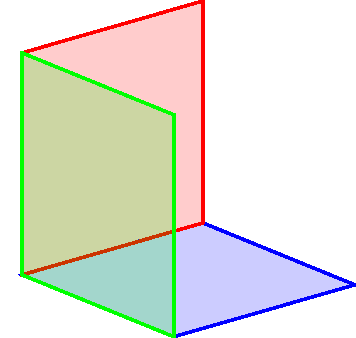
\includegraphics[width=\textwidth]{figures/3/manifold_a.pdf}
	\caption{Three perpendicular walls.}
	\label{fig:manifold_a}
\end{subfigure} \hfill%
\begin{subfigure}{0.45\textwidth}
	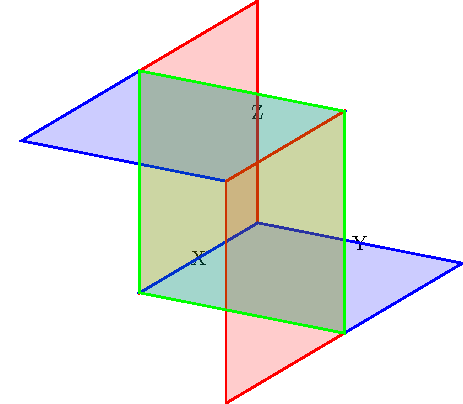
\includegraphics[width=\textwidth]{figures/3/manifold_b.pdf}
	\caption{Five perpendicular walls.}
	\label{fig:manifold_b}
\end{subfigure}
\caption{Two types of manifold used in our constructions.}
\label{fig:manifold_types}
\end{figure} 

%The set $M$, obtained from the union of mutually orthogonal faces of $G$, 
It bears mention that many lethal sets on manifolds are discovered through trial and error. One strategy is to imagine these manifolds as folded pieces of paper, and to identify lethal sets on their unfolded nets. This technique is discussed in more detail in Chapter \{CONSTRUCTIONS\}. 

\end{comment}
